\section{Phenomenological Pipeline}

The estimation of signal and background event yields is performed through a comprehensive Monte Carlo (MC) simulation pipeline~\cite{Christensen:2008py,Alloul:2013bka,Degrande:2011ua,Alwall:2014hca}. This approach, a cornerstone of high-energy physics research, enables robust studies of Beyond the Standard Model (BSM) scenarios by emulating the entire data collection and processing chain of a collider experiment~\cite{Sjostrand:2014zea,deFavereau:2013fsa}. The key advantages of this methodology include~\cite{Alwall:2014hca,Cacciari:2011ma}:

\begin{itemize}
    \item The ability to perform automated calculations of theoretical quantities such as cross-sections and decay widths for complex processes.
    \item Conducting feasibility studies and optimizing analysis strategies prior to data acquisition.
    \item Estimating the efficiency of complex event selection criteria and the geometric acceptance of the detector.
    \item Predicting the rates and kinematical distributions of both irreducible and reducible background processes.
    \item Comparing and distinguishing between different theoretical hypotheses for a potential discovered signal.
\end{itemize}

The simulation workflow is modular, reflecting the logical progression from a theoretical Lagrangian to simulated detector-level observables~\cite{Christensen:2008py,Alloul:2013bka,Degrande:2011ua,Alwall:2014hca}. A schematic view of this pipeline is presented in Figure~\ref{fig:sim_workflow}~\cite{Alwall:2014hca,deFavereau:2013fsa}.

\begin{center}
    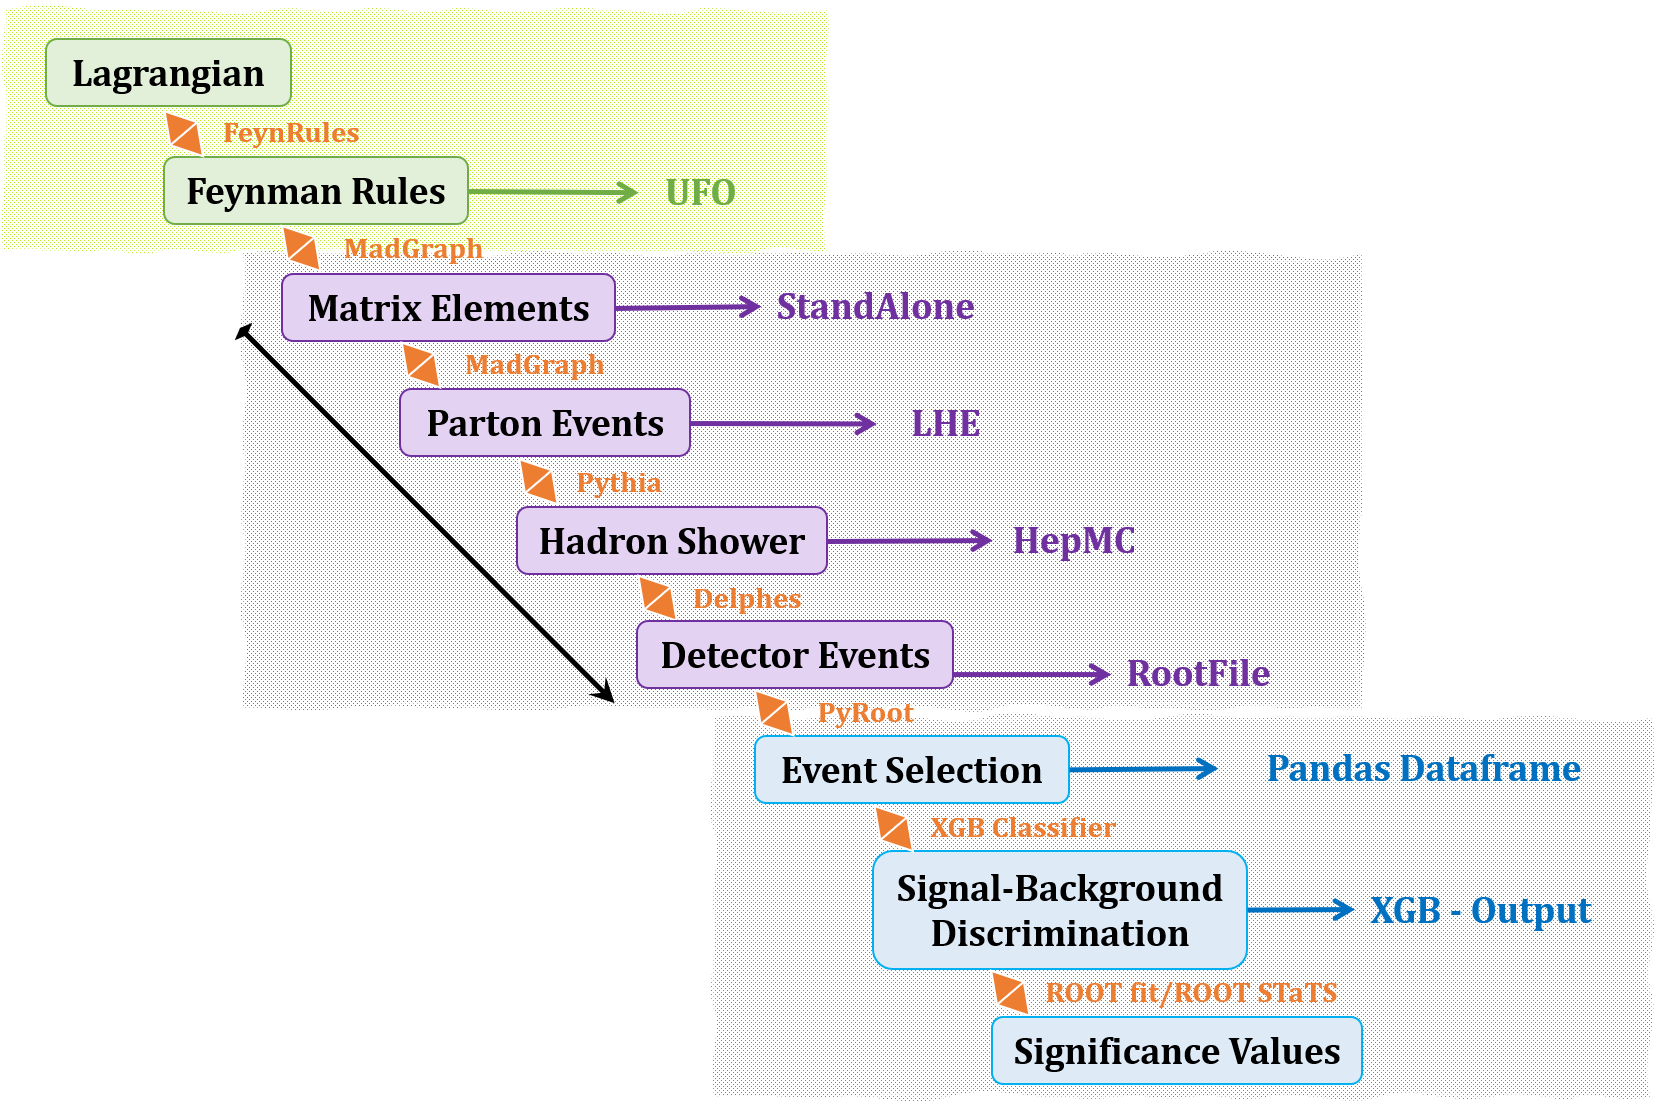
\includegraphics[width=\textwidth]{Slides/2023_paper/Workflow.png}
    \captionof{figure}{Schematic overview of the phenomenological MC pipeline: model definition (FeynRules) -> UFO export -> matrix-element generation (MadGraph) -> parton shower and hadronization (PYTHIA) -> fast detector simulation (DELPHES) -> analysis ntuples (ROOT).}\label{fig:sim_workflow}
\end{center}

The process begins with the implementation of the theoretical model in \texttt{FeynRules} (v2.3.43)~\parencite{Christensen:2008py,Alloul:2013bka}. The Lagrangian of the new physics scenario, including all particle definitions, parameters, and interactions, is translated into a set of Feynman rules and exported in the Universal FeynRules Output (UFO) format~\cite{Degrande:2011ua}, interoperable with modern matrix-element generators~\cite{Alwall:2014hca}.

This UFO module, accompanied by a parameter card defining numerical values for masses and couplings, serves as input to \texttt{MadGraph5\_aMC@NLO} (v3.5.7)~\parencite{Alwall:2014bza,Alwall:2014hca}. Within MadGraph the hard process and corresponding matrix elements are generated and stored in Les Houches event (LHE) files; PDF choices (here NNPDF3.0 NLO~\parencite{NNPDF:2014otw}) and matching/merging settings (MLM/CKKW-type) are configured to control radiation and multi-jet overlap~\cite{Alwall:2007fs,Buckley:2015}. Parton-level LHE events are passed to \texttt{PYTHIA 8} for showering, hadronization and decays~\parencite{Sjostrand:2014zea}, and the generator output is exchanged in HepMC format for downstream processing~\cite{Dobbs:2001}.

To accurately model processes featuring significant interference effects between the new physics signal (e.g., a $\zb'$ boson) and the Standard Model backgrounds, the full squared amplitude (often referred to as the Signal-Discriminated Events or SDE strategy) is employed for the phase-space integration. The \texttt{MadEvent} submodule then generates unweighted parton-level events, which are stored in the Les Houches Event (LHE) format, containing the four-momenta of all final-state particles. The generation is optimized through careful configuration of the \texttt{run\_card}, setting appropriate kinematic cuts on final-state partons to avoid wasting computational resources on events that would subsequently be rejected by the detector simulation.

Given the presence of additional jet radiation, the MLM matching scheme~\parencite{Alwall:2007fs} is applied to mitigate the double-counting of jet emission between the matrix element calculation and the subsequent parton shower. This ensures a smooth transition between the hard process and softer radiative effects.

The parton-level LHE events are then passed to \texttt{PYTHIA} (v8.2.44)~\parencite{Sjostrand:2014zea} for the modeling of QCD and QED radiation (parton showering), hadronization, and particle decays. This step translates the colored partons into stable, color-singlet hadrons and resonances that form the observable final state. The resulting events, which include a full list of generator-level particles, are saved in the HepMC2 format.

Detector effects are simulated using \texttt{DELPHES} (v3.4.2)~\parencite{deFavereau:2013fsa}, a fast parametric detector simulation framework. The \texttt{delphes\_card\_CMS.tcl} configuration card is used to emulate the response of the CMS detector, including the geometric acceptance, tracking efficiency, calorimeter energy resolution and segmentation, and magnetic field. Key reconstruction algorithms are applied within DELPHES:
\begin{itemize}
    \item Jets are clustered from calorimeter towers using the anti-$k_t$ algorithm~\parencite{Cacciari:2008gp} with a distance parameter of $R=0.4$, and $b$-tagging is simulated based on the efficiency and mis-tag rate of the CMS performance.
    \item Muons and electrons are identified with efficiency maps that are functions of $p_T$ and $\eta$.
    \item The missing transverse energy (MET) is calculated from the negative vector sum of all reconstructed particle momenta.
\end{itemize}
The final output, containing reconstructed physics objects (jets, leptons, MET), is stored in ROOT format~\parencite{Brun:1997pa}.

At this stage, the analysis of the simulated samples converges with the methodology applied to real collider data. The subsequent steps involve applying event selection criteria, calibrating and scaling the reconstructed objects (e.g., applying Jet Energy Corrections), and performing statistical interpretation. The reliability of the simulation is validated by comparing the modeling of well-known Standard Model processes (e.g., Drell-Yan, $t\bar{t}$ production) against published results and data-driven control regions. Dominant theoretical systematic uncertainties, such as those arising from the choice of factorization and renormalization scales, PDF variations, and parton shower modeling, are evaluated and propagated through the analysis.

